\documentclass[letterpaper,12pt]{article}
\usepackage{enumitem}
\usepackage[utf8]{inputenc}
\usepackage{amsmath}
\usepackage[T1]{fontenc}
\usepackage{geometry}
\geometry{margin=2.5cm}
\usepackage{lmodern}
\usepackage{dirtytalk}
\usepackage{graphicx}
\usepackage{mathtools}
\usepackage{mathrsfs}
\usepackage{float}
\let\lll\relax
\usepackage{amssymb}
\usepackage{bbm}
\usepackage{amsthm}
\usepackage{hyperref}
\usepackage{cleveref}
\usepackage{indentfirst}
\usepackage{microtype}
\binoppenalty=10000
\relpenalty=10000
\setlength{\emergencystretch}{3em}
\usepackage{listings}
\usepackage{xcolor}
\usepackage[numbers]{natbib}
\newtheorem{lemma}{Lemma}
\allowdisplaybreaks

\title{Proof for Diamond Graph $G$}
\author{Zofia Kuriata}
\date{2026-09-09}

\begin{document}

\maketitle
\tableofcontents
\newpage

\section{Problem}
We would like to prove that $0.54413127767139846114$ is the value of $\text{mod}(G)$ and it is achieved by a partition where four clusters have $184$ diamonds and $1$ path vertex, and the rest of the diamonds have their own clusters --- Figure~\ref{best_mod}.

\begin{figure}[H]
      \centering
      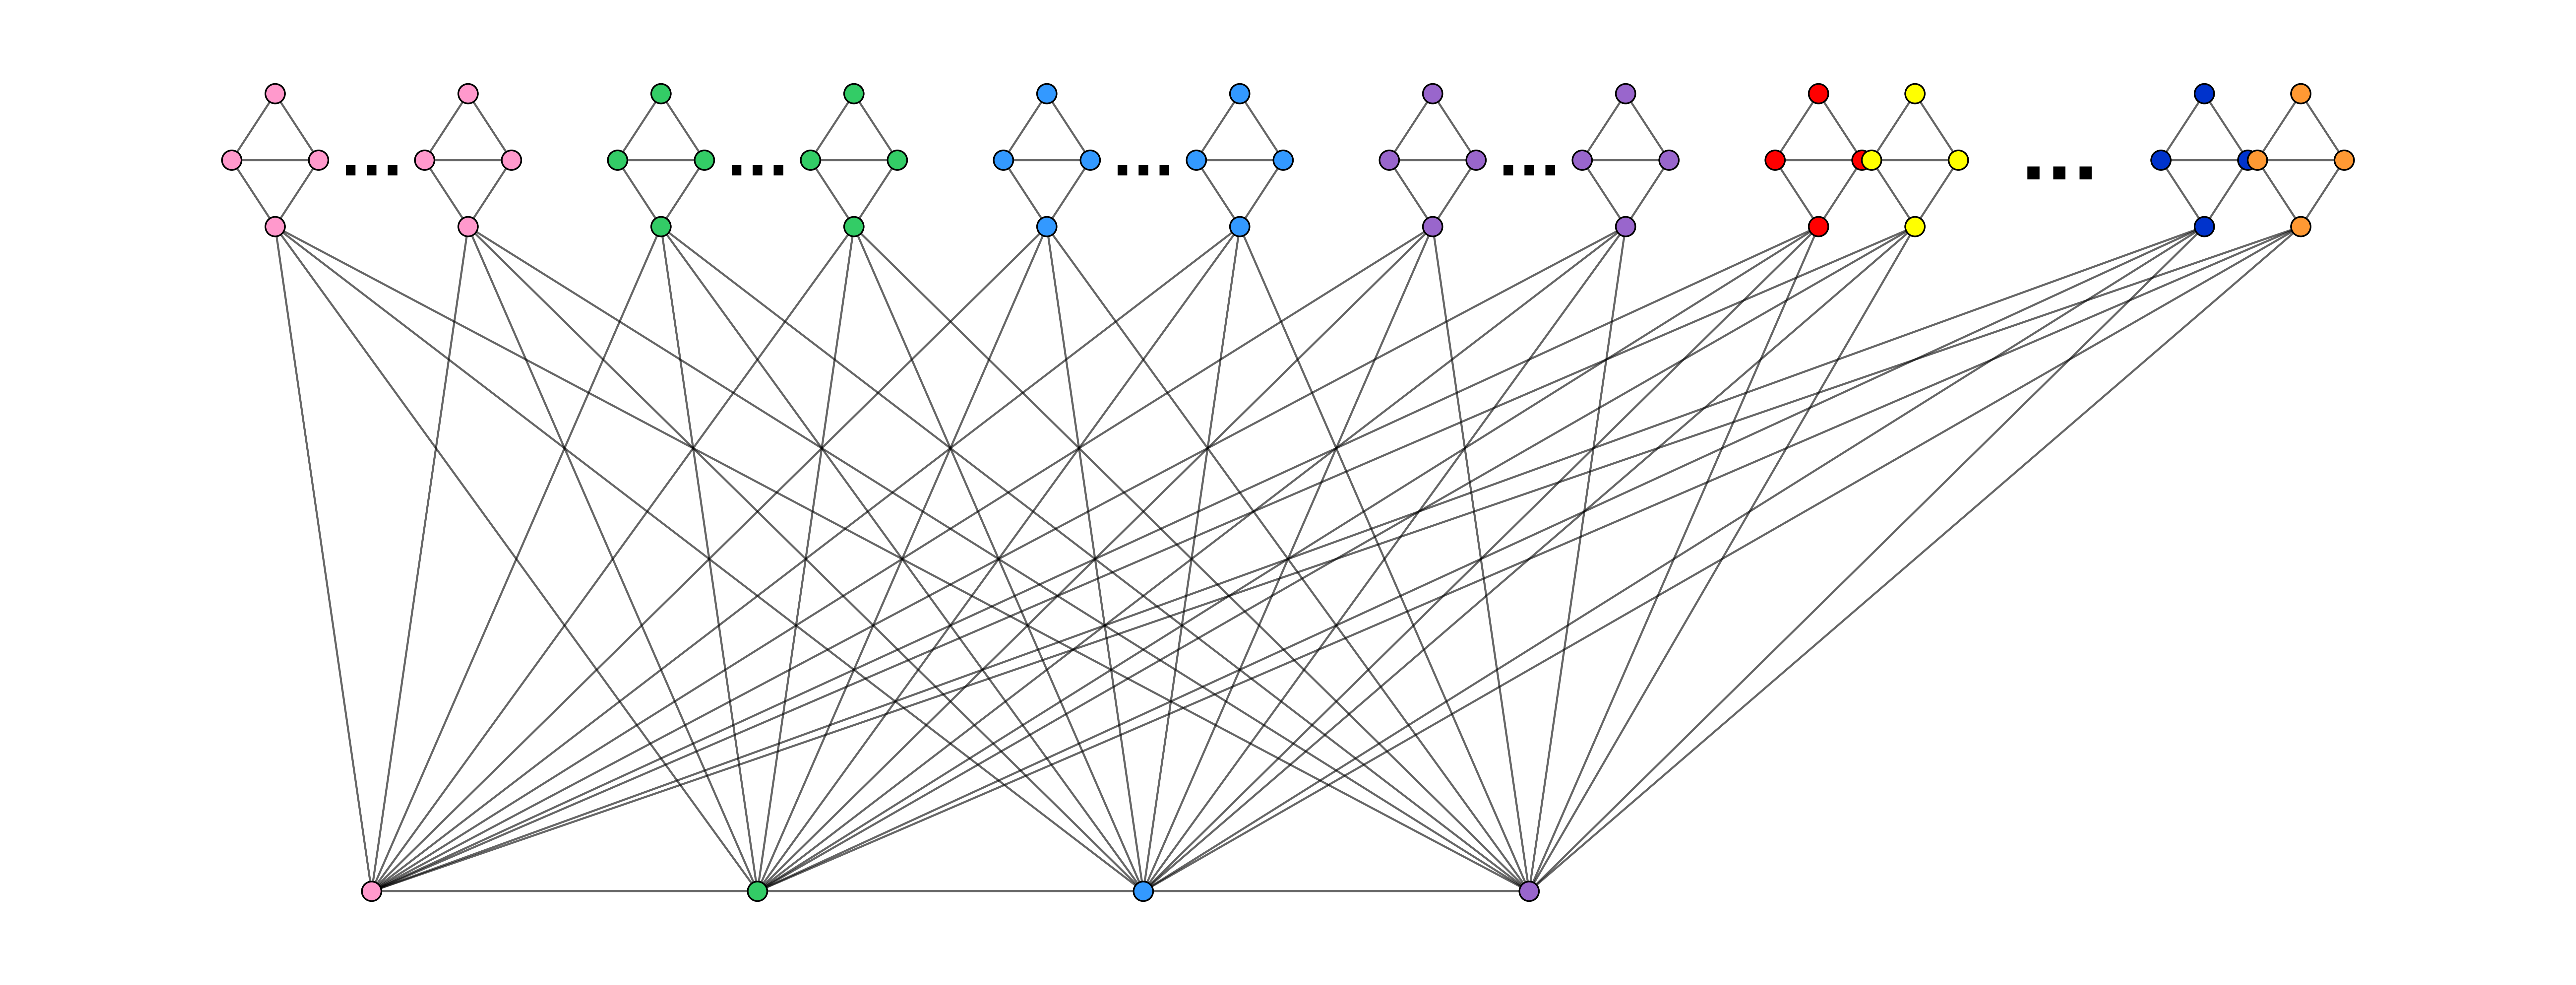
\includegraphics[width=0.9\textwidth]{../../graphs/best_mod.png}
      \caption{The best found clustering for modularity.}
      \label{best_mod}
\end{figure}

If we proved it, we would also prove that there indeed exists a graph $G$ such that $\text{mod}^*(G) > \text{mod}(G)$, which is our \textit{diamond graph G}.

\section{Definitions and Notation}
Let $G = (V, E)$ be the considered diamond graph and $m = |E| = 81003$ be the total number of edges in $G$.
\begin{itemize}
      \item $d_i$ --- the $i$-th diamond subgraph (where $e(d_i) = 5$ and $\text{vol}(d_i) = 14$),
      \item $t_i$ --- the $i$-th top triangle of diamond $d_i$,
      \item $c_i$ --- the connector vertex of $i$-th diamond attached to the path,
      \item $p_1, p_2, p_3, p_4$ --- vertices forming the central path (path vertices),
      \item $\text{vol}(C) = \sum_{v \in C} \deg(v)$ --- the volume of cluster $C$ (sum of degrees of vertices in $C$),
      \item $e(C)$ --- the number of internal edges in cluster $C$,
      \item $\text{mod}_{\mathcal{C}}(G) = \sum_{C \in \mathcal{C}} \left[ \frac{e(C)}{m} - \left(\frac{\text{vol}(C)}{2m}\right)^2 \right]$ --- modularity of graph $G$ under partition $\mathcal{C}$,
      \item $\mathcal{A}$ --- partition shown in Figure~\ref{best_mod} scoring $0.54413127767139846114$,
      \item $A_1, A_2, A_3, A_4$ --- clusters in $\mathcal{A}$ containing $184$ diamonds and $1$ path vertex each,
      \item $A_5, \ldots, A_{8268}$ --- clusters in $\mathcal{A}$ containing exactly $1$ standalone diamond.
\end{itemize}

\begin{lemma}\label{positive_score}
      Let \(G = (V,E)\) be a graph and \(\mathcal{A}\) be a partition of vertices of \(G\) such that \(mod_{\mathcal{A}}(G) = mod(G)\). Then \(\forall_{A \in \mathcal{A}} \hspace{1mm} mod_A(G) \geq 0\).
\end{lemma}

\begin{lemma}\label{connected_clusters}
      Let \(G = (V,E)\) be a graph and \(\mathcal{A}\) be a partition of vertices of \(G\) such that \(mod_{\mathcal{A}}(G) = mod(G)\). Then every community in partition \(\mathcal{A}\) induces a connected subgraph.
\end{lemma}


\section{Structural Analysis}
\subsection{Splitting Triangles and Diamonds}
First, we will show that there is no point in splitting the top triangle in each diamond. Let $a,b,c$ be vertices of a triangle such that $deg(c)=2$. At first, let's take a look at the case when the vertex $a$ (or symmetrically $b$) is in a different community than $b$ and $c$. There are three main scenarios for such clustering.
\begin{enumerate}
      \item $a,b,c$ are in separate clusters.\\
            Let's notice that if $c$ is grouped neither with $b$ nor $a$, then it must be in its own one-vertex community (Lemma \ref{connected_clusters}). Similarly for $a$ and $b$ - if they are not together, then at least one of them also must be alone (because there is only one remaining neighbour of them -- the connector), let's assume that $a$ is alone. Let $C_1 = \{c\}, C_2 = \{a\}, C_1' = \emptyset$ and $C_2' = \{a,c\}$. We will show that joining $C_1$ and $C_2$ will increase mod score
            \begin{align*}
                   & \text{mod}_{\mathcal{C'}}(G) - \text{mod}_{\mathcal{C}} (G) \\
                   & = \frac{1}{m} - \frac{5^2}{4m^2} + \frac{2^2 + 3^2}{4m^2}   \\
                   & = \frac{4m-25+4+9}{4m^2}                                    \\
                   & = \frac{4m-12}{4m^2} > 0.                                   \\
            \end{align*}
            \begin{figure}[H]
                  \centering
                  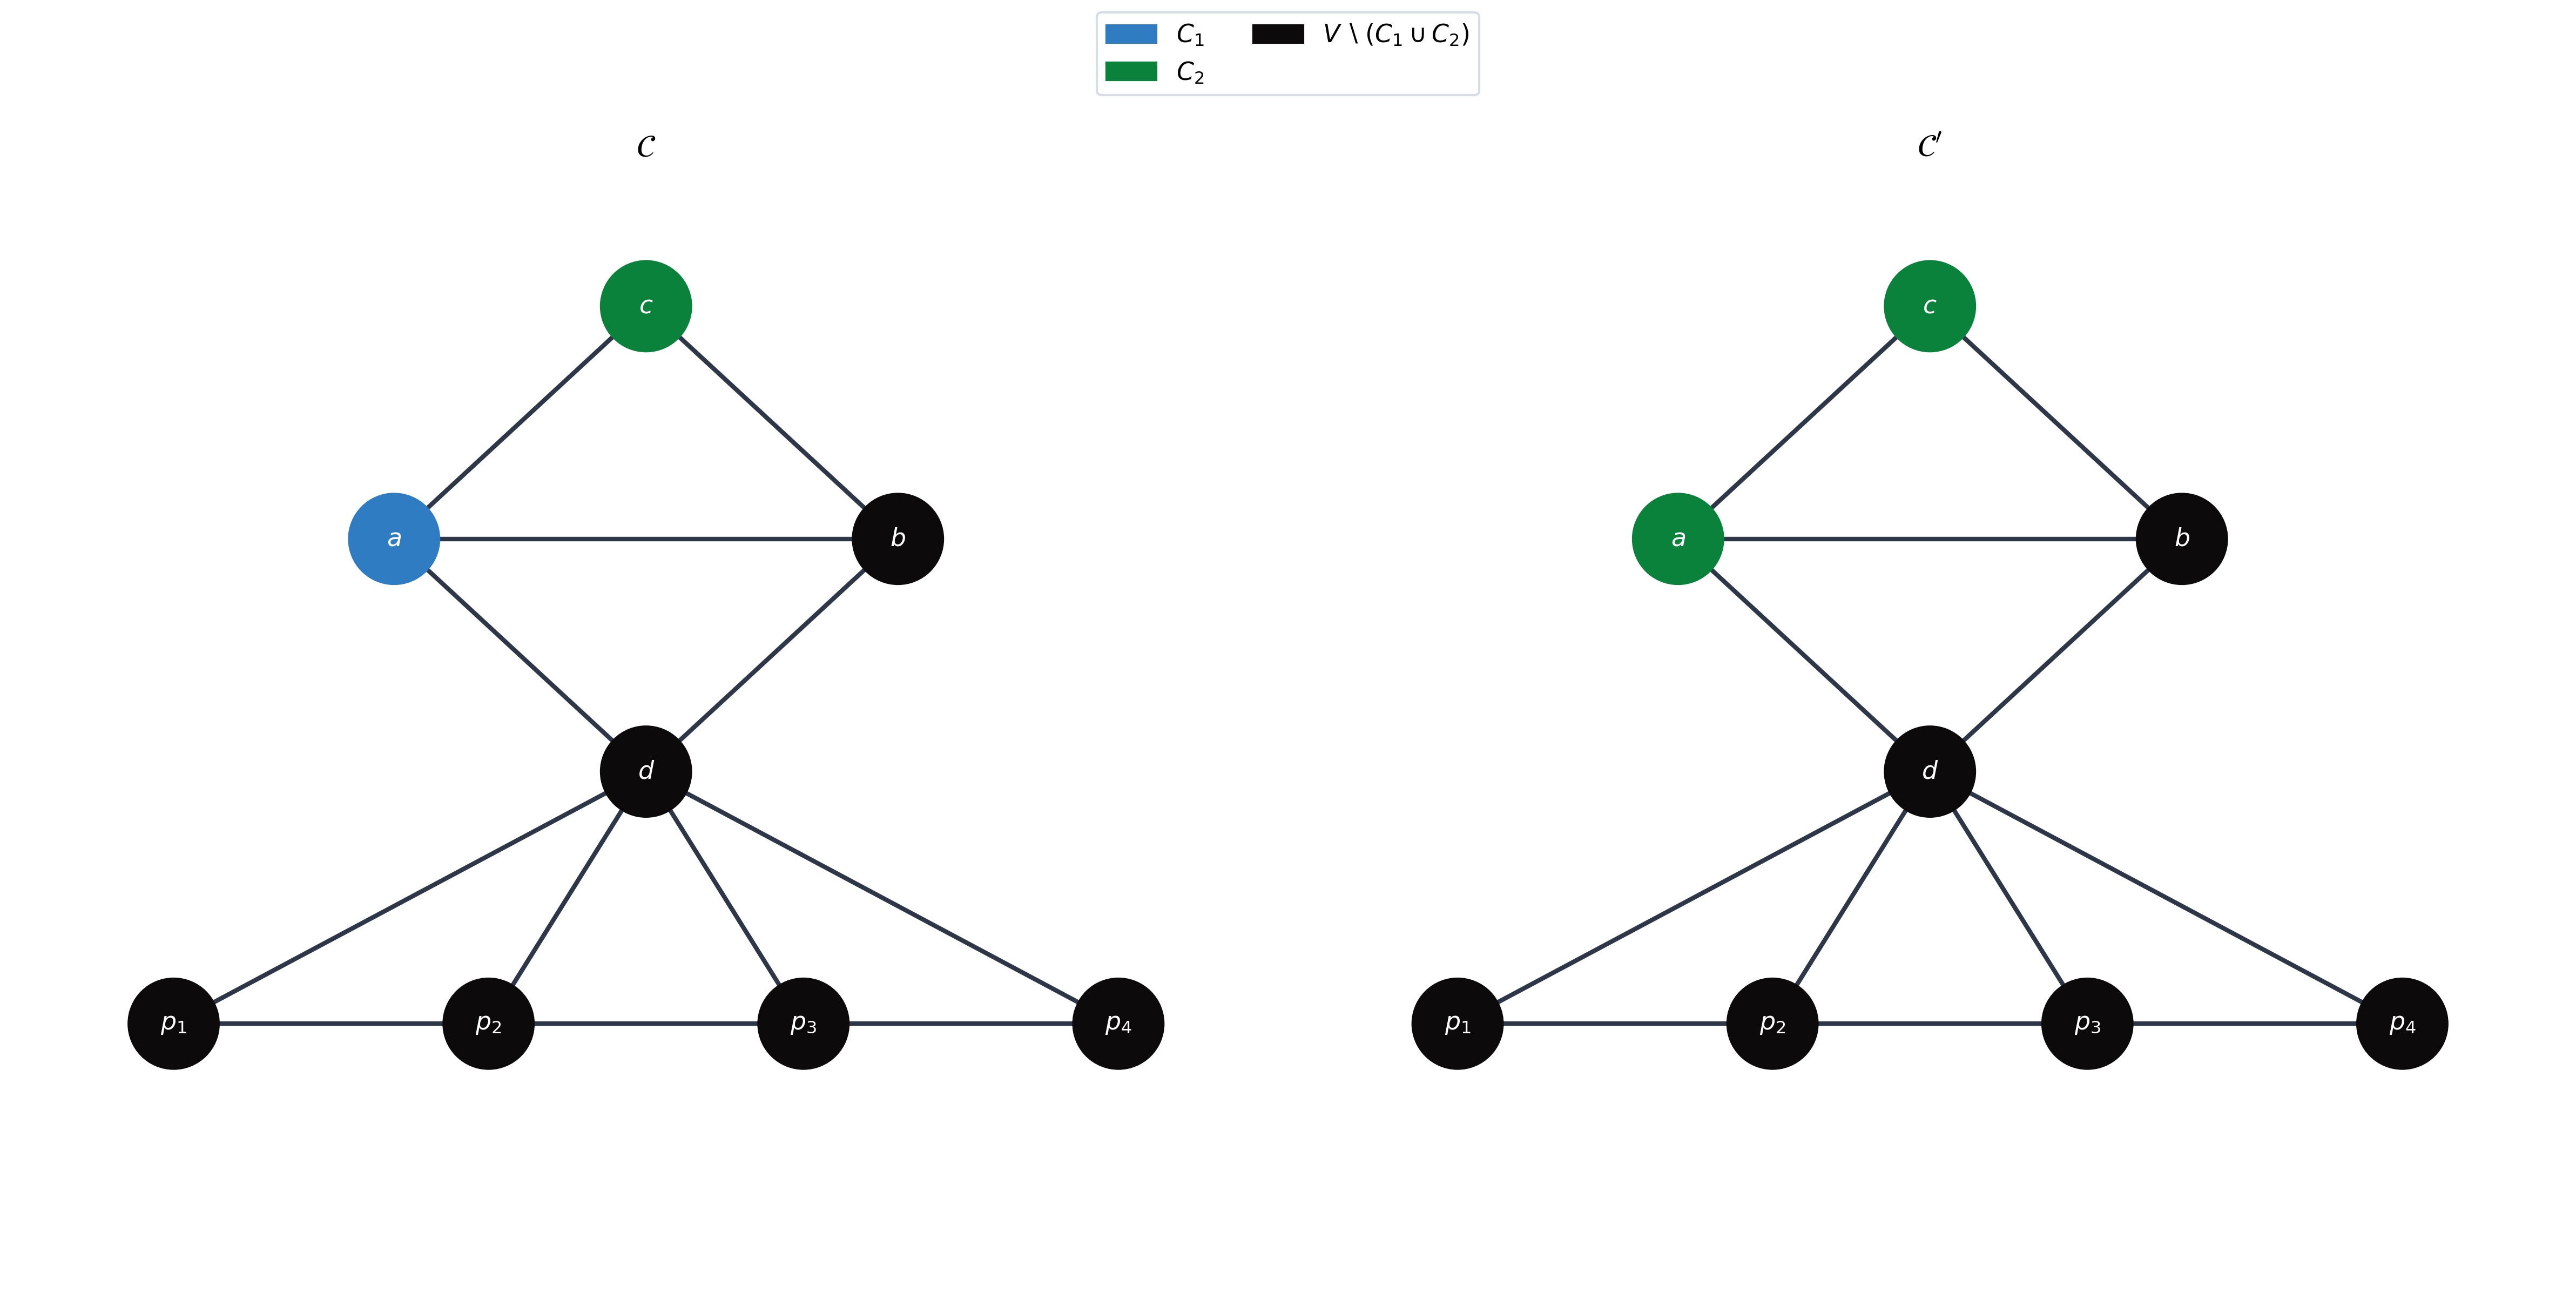
\includegraphics[width=0.7\textwidth]{../../graphs/t1.png}
                  \caption{Merging two alone triangle vertices.}
                  \label{fig:t1}
            \end{figure}
            Therefore in optimal partitioning, no triangle can be split into three clusters.\\
      \item $a,c$ together, $b$ in a separate cluster.\\
            We need to consider three scenarios, depending on where the connector is located.
            \begin{enumerate}[label=(\alph*)]
                  \item Connector ($d$) is in $b's$ cluster.\\
                        Let $b,d \in C_1, C_2 = \{a,c\}, C_1' = C_1 \setminus \{b\}$ and $C_2' = \{a,c,b\}$. The difference is
                        \begin{align*}
                               & \text{mod}_{\mathcal{C'}}(G) - \text{mod}_{\mathcal{C}} (G)                        \\
                               & = \frac{2}{m} - \frac{1}{m} - \frac{-6vol(C_1)+9}{4m^2} - \frac{6vol(C_2)+9}{4m^2} \\
                               & = \frac{4m+6vol(C_1)-6\cdot 5-18}{4m^2}                                            \\
                               & = \frac{4m+6vol(C_1)-48}{4m^2} > 0.                                                \\
                        \end{align*}
                        \begin{figure}[H]
                              \centering
                              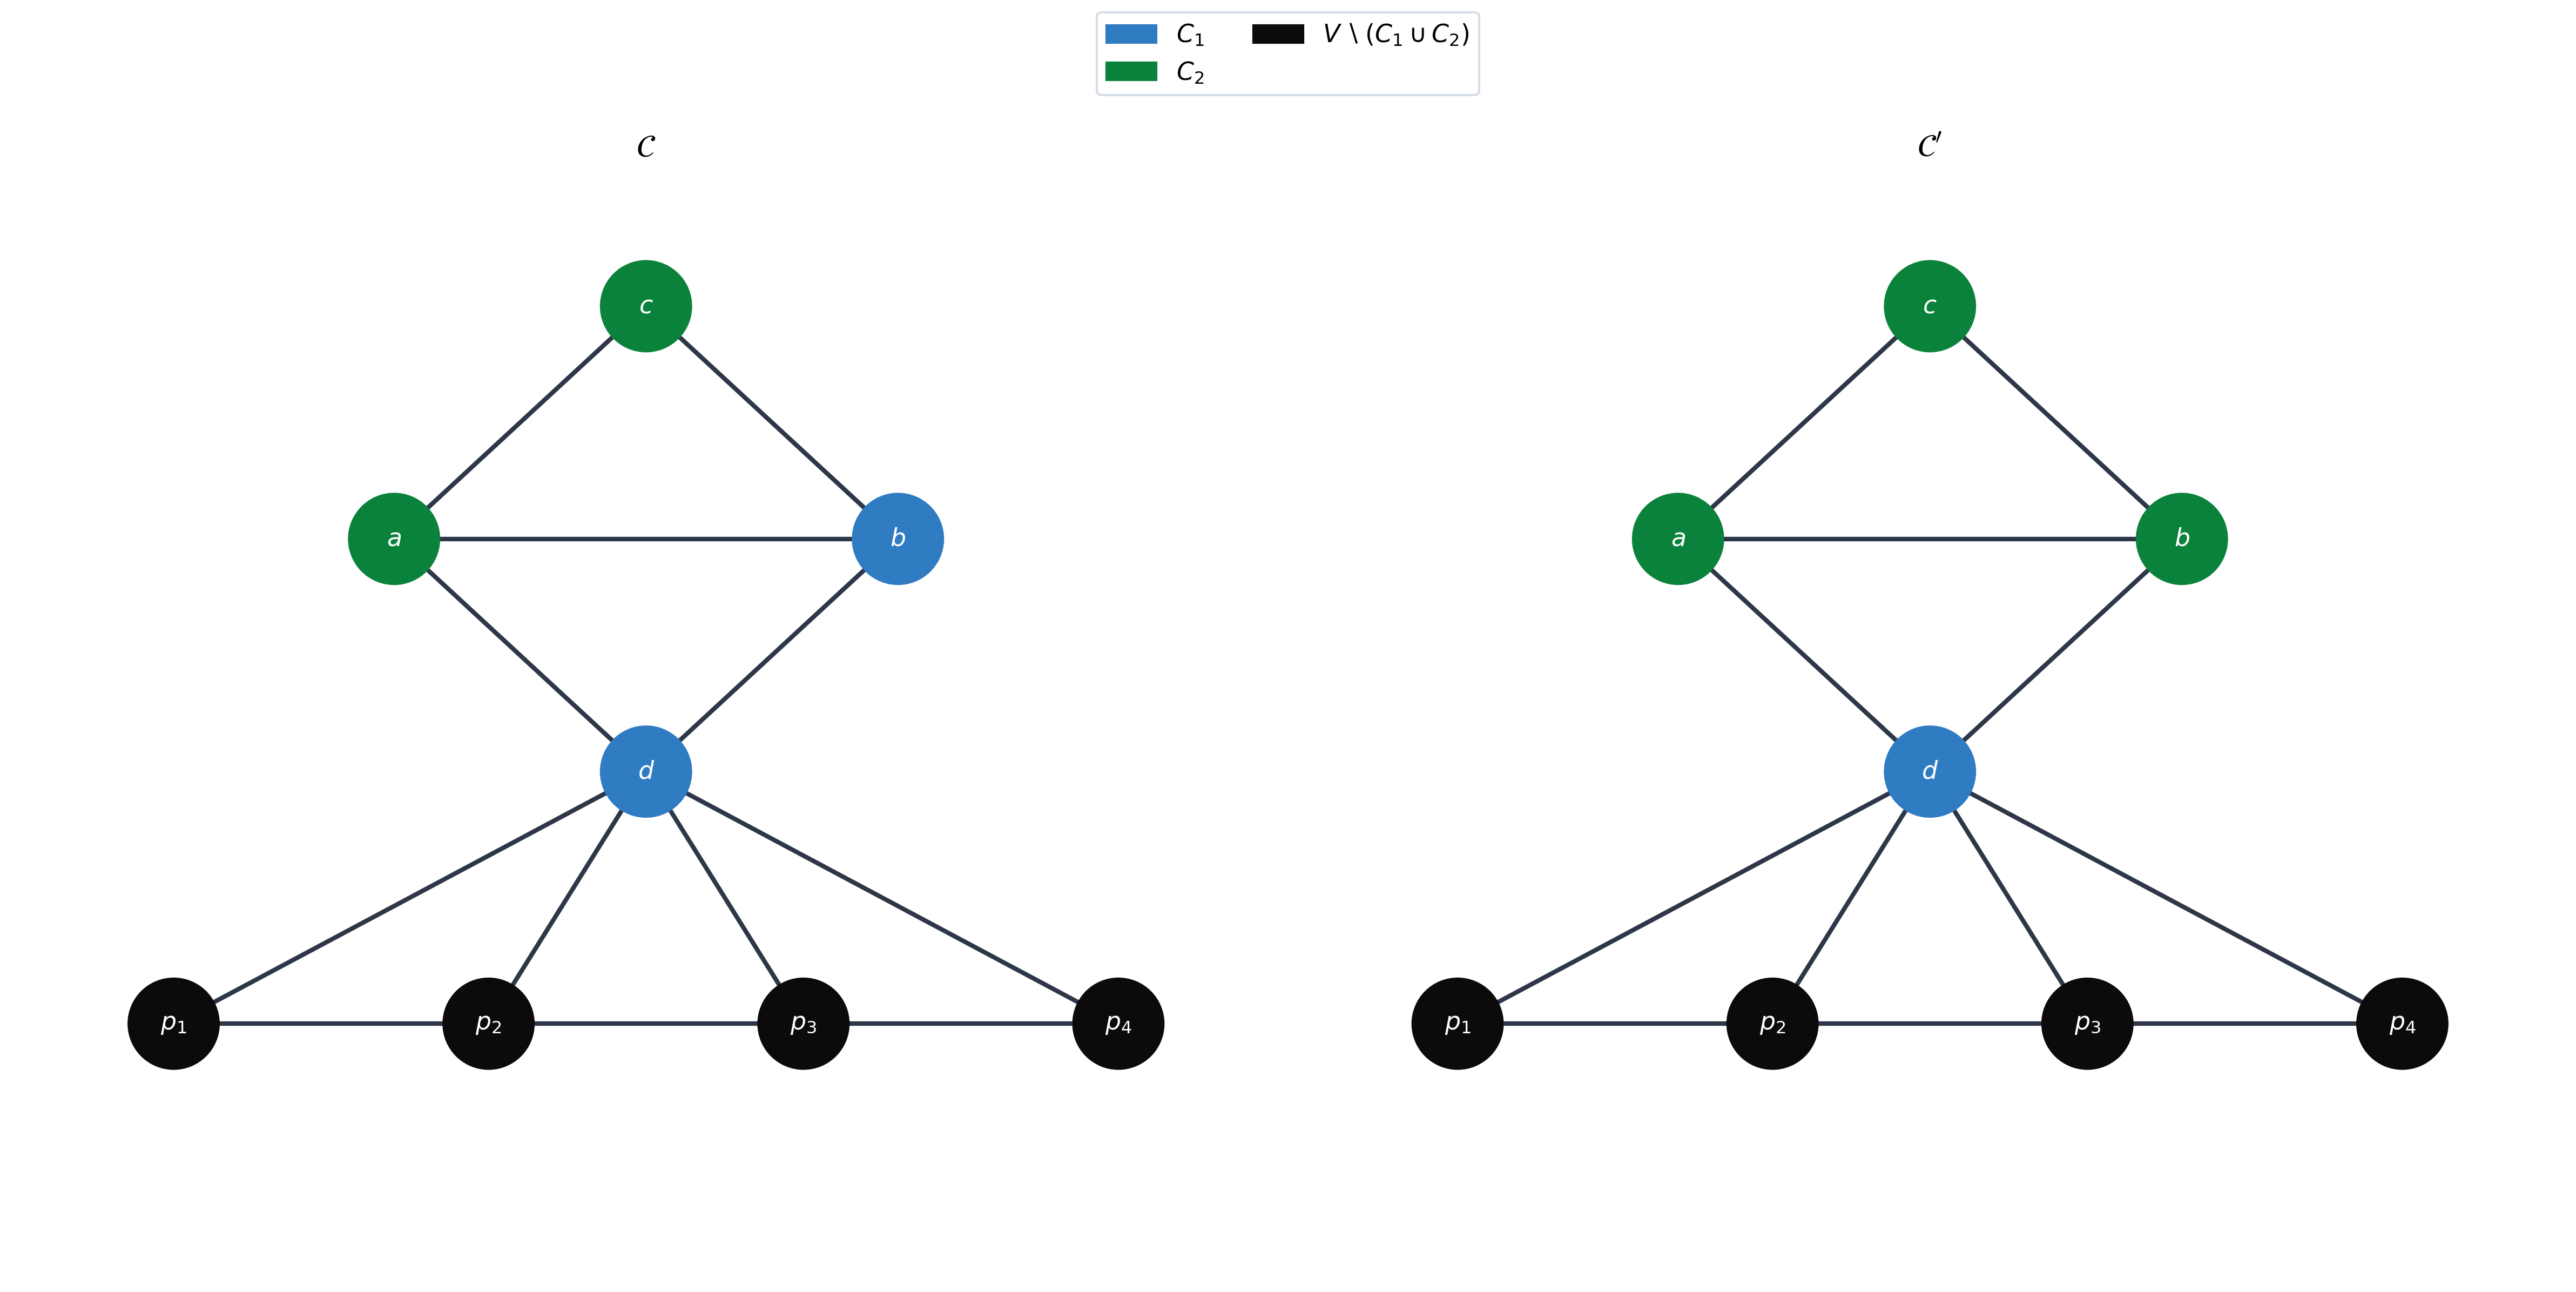
\includegraphics[width=0.7\textwidth]{../../graphs/t2a.png}
                              \caption{Moving b from the connector to the triangle.}
                              \label{fig:t2a}
                        \end{figure}
                  \item Connector ($d$) is in the cluster containing $a,c$ ($b$ is alone).\\
                        Let $C_1 = \{b\}, a,c,d \in C_2, C_1' = \emptyset$ and $C_2' = C_2 \cup \{b\}$. The difference is
                        \begin{align*}
                               & \text{mod}_{\mathcal{C'}}(G) - \text{mod}_{\mathcal{C}} (G) \\
                               & = \frac{3}{m} - \frac{6vol(C_2)+9}{4m^2} + \frac{9}{4m^2}   \\
                               & = \frac{12m-6vol(C_2)}{4m^2} \geq 0.                        \\
                        \end{align*}
                        \begin{figure}[H]
                              \centering
                              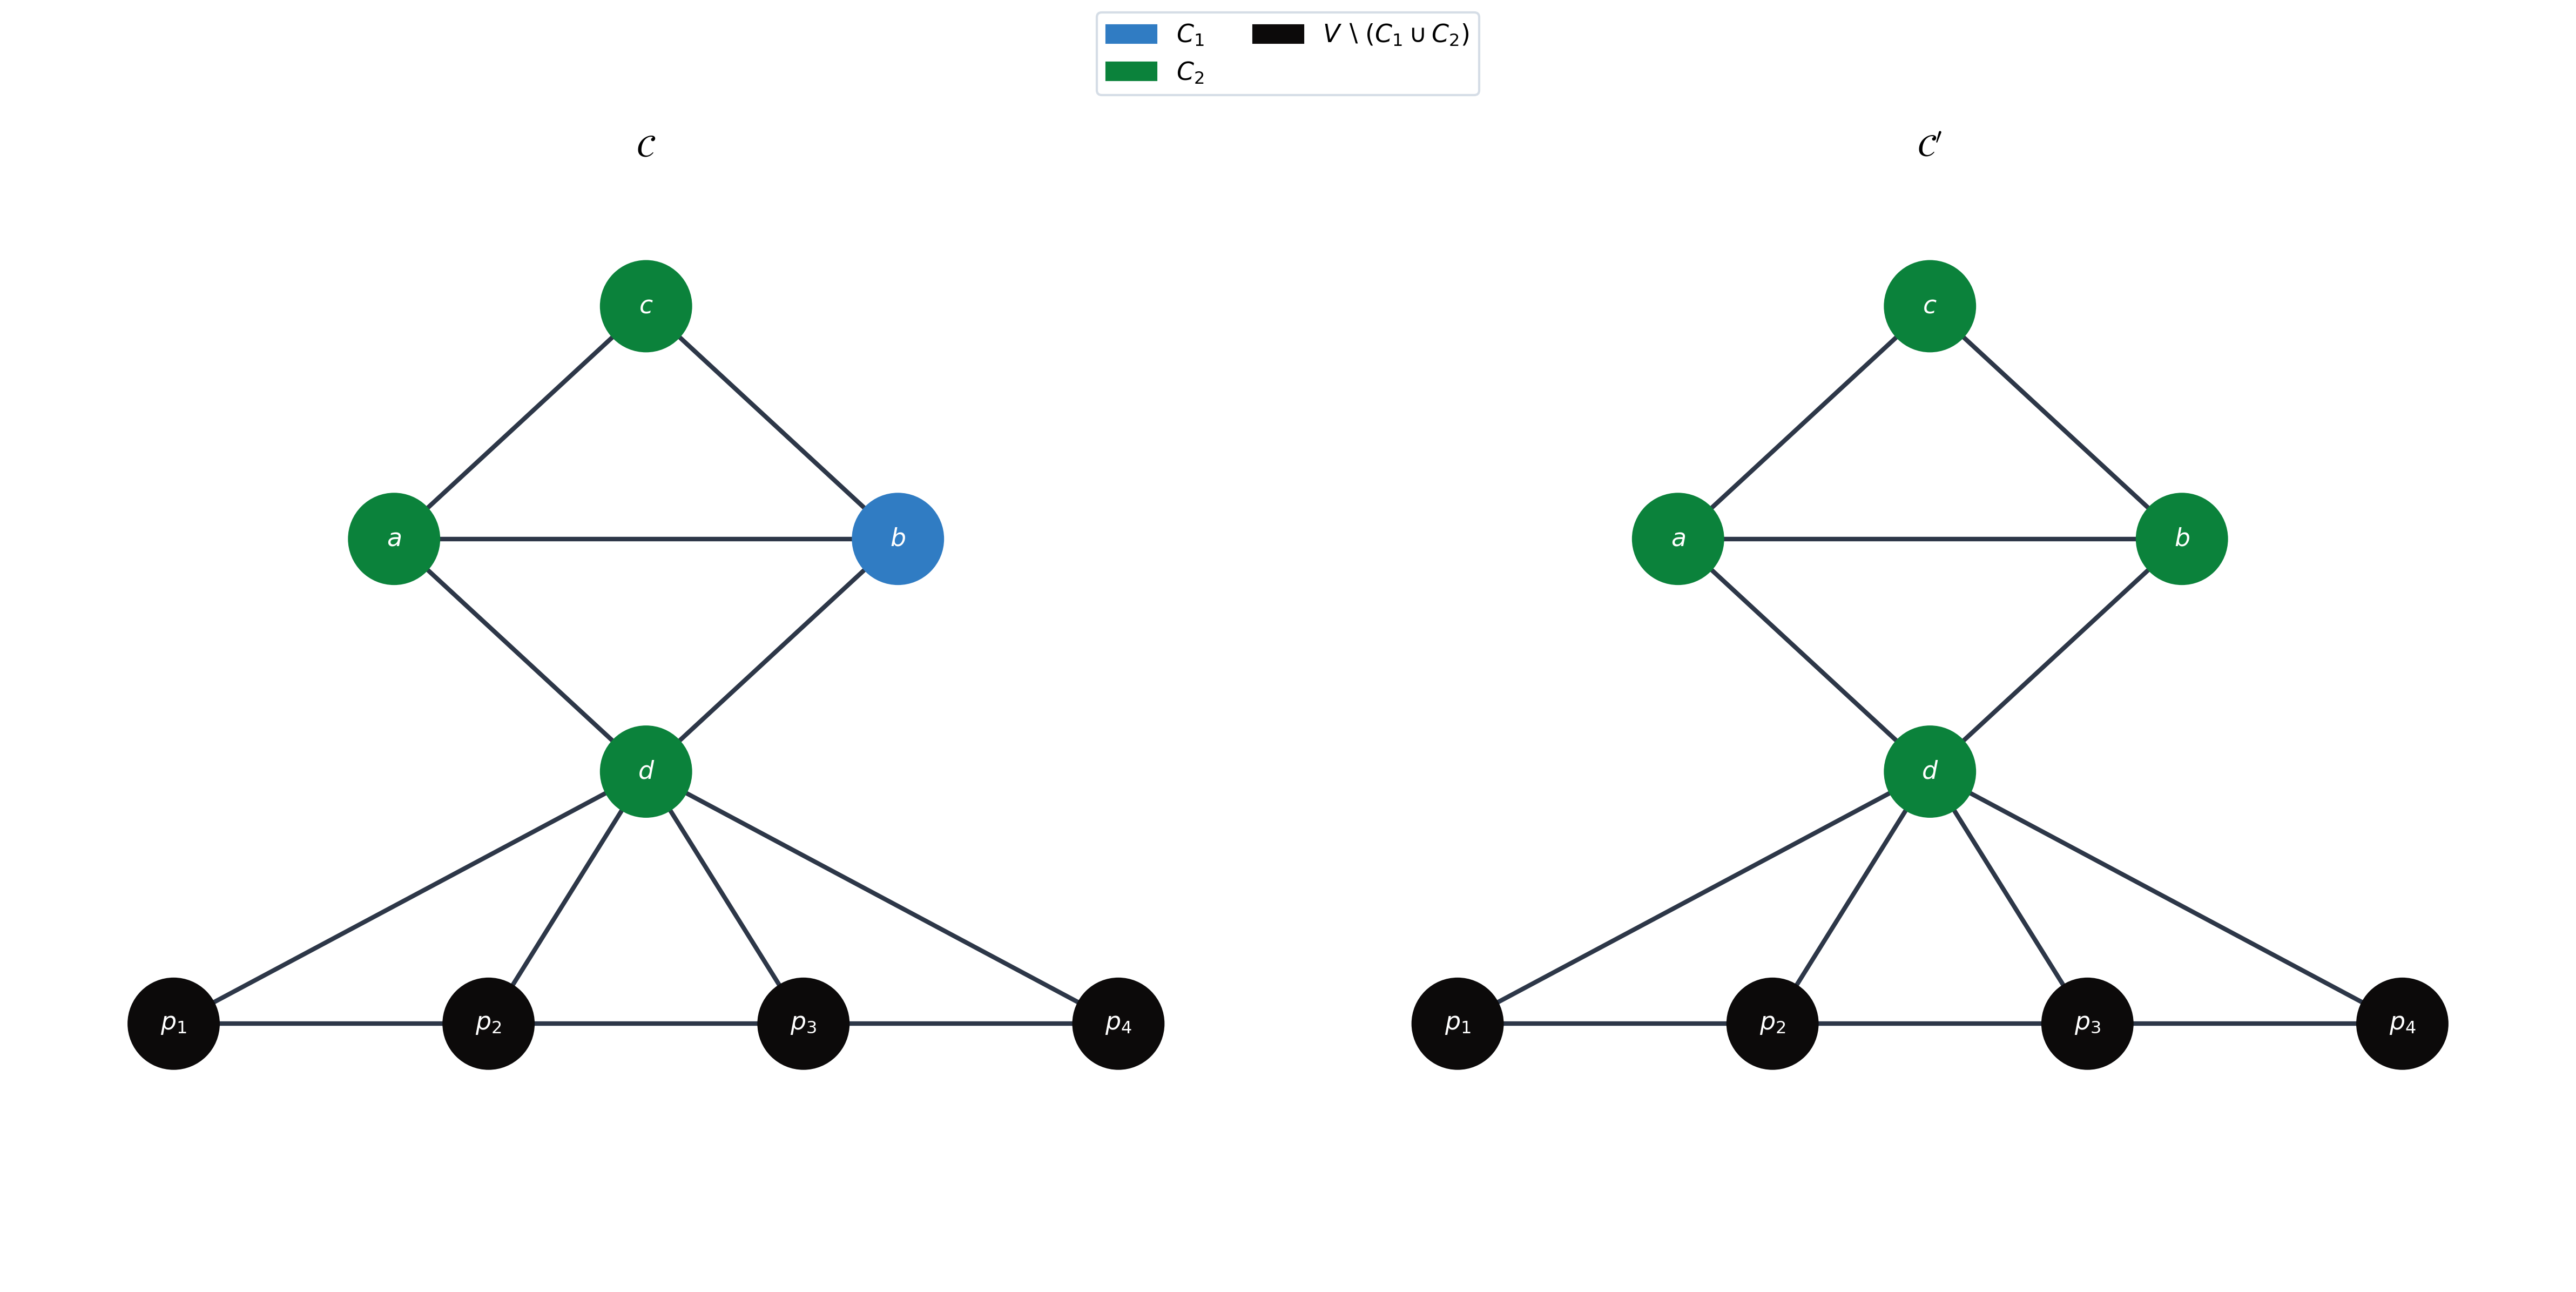
\includegraphics[width=0.7\textwidth]{../../graphs/t2b.png}
                              \caption{Moving b to the whole diamnod.}
                              \label{fig:t2b}
                        \end{figure}
                  \item Connector is in a separate cluster.\\
                        Let $C_1 = \{b\}, C_2 = \{a,c\}, C_1' = \emptyset$ and $C_2' = \{a,c,b\}$. The difference is
                        \begin{align*}
                               & \text{mod}_{\mathcal{C'}}(G) - \text{mod}_{\mathcal{C}} (G) \\
                               & = \frac{2}{m} - \frac{6vol(C_2)+9}{4m^2} + \frac{9}{4m^2}   \\
                               & = \frac{8m-6\cdot 5}{4m^2} > 0.                             \\
                        \end{align*}
                        \begin{figure}[H]
                              \centering
                              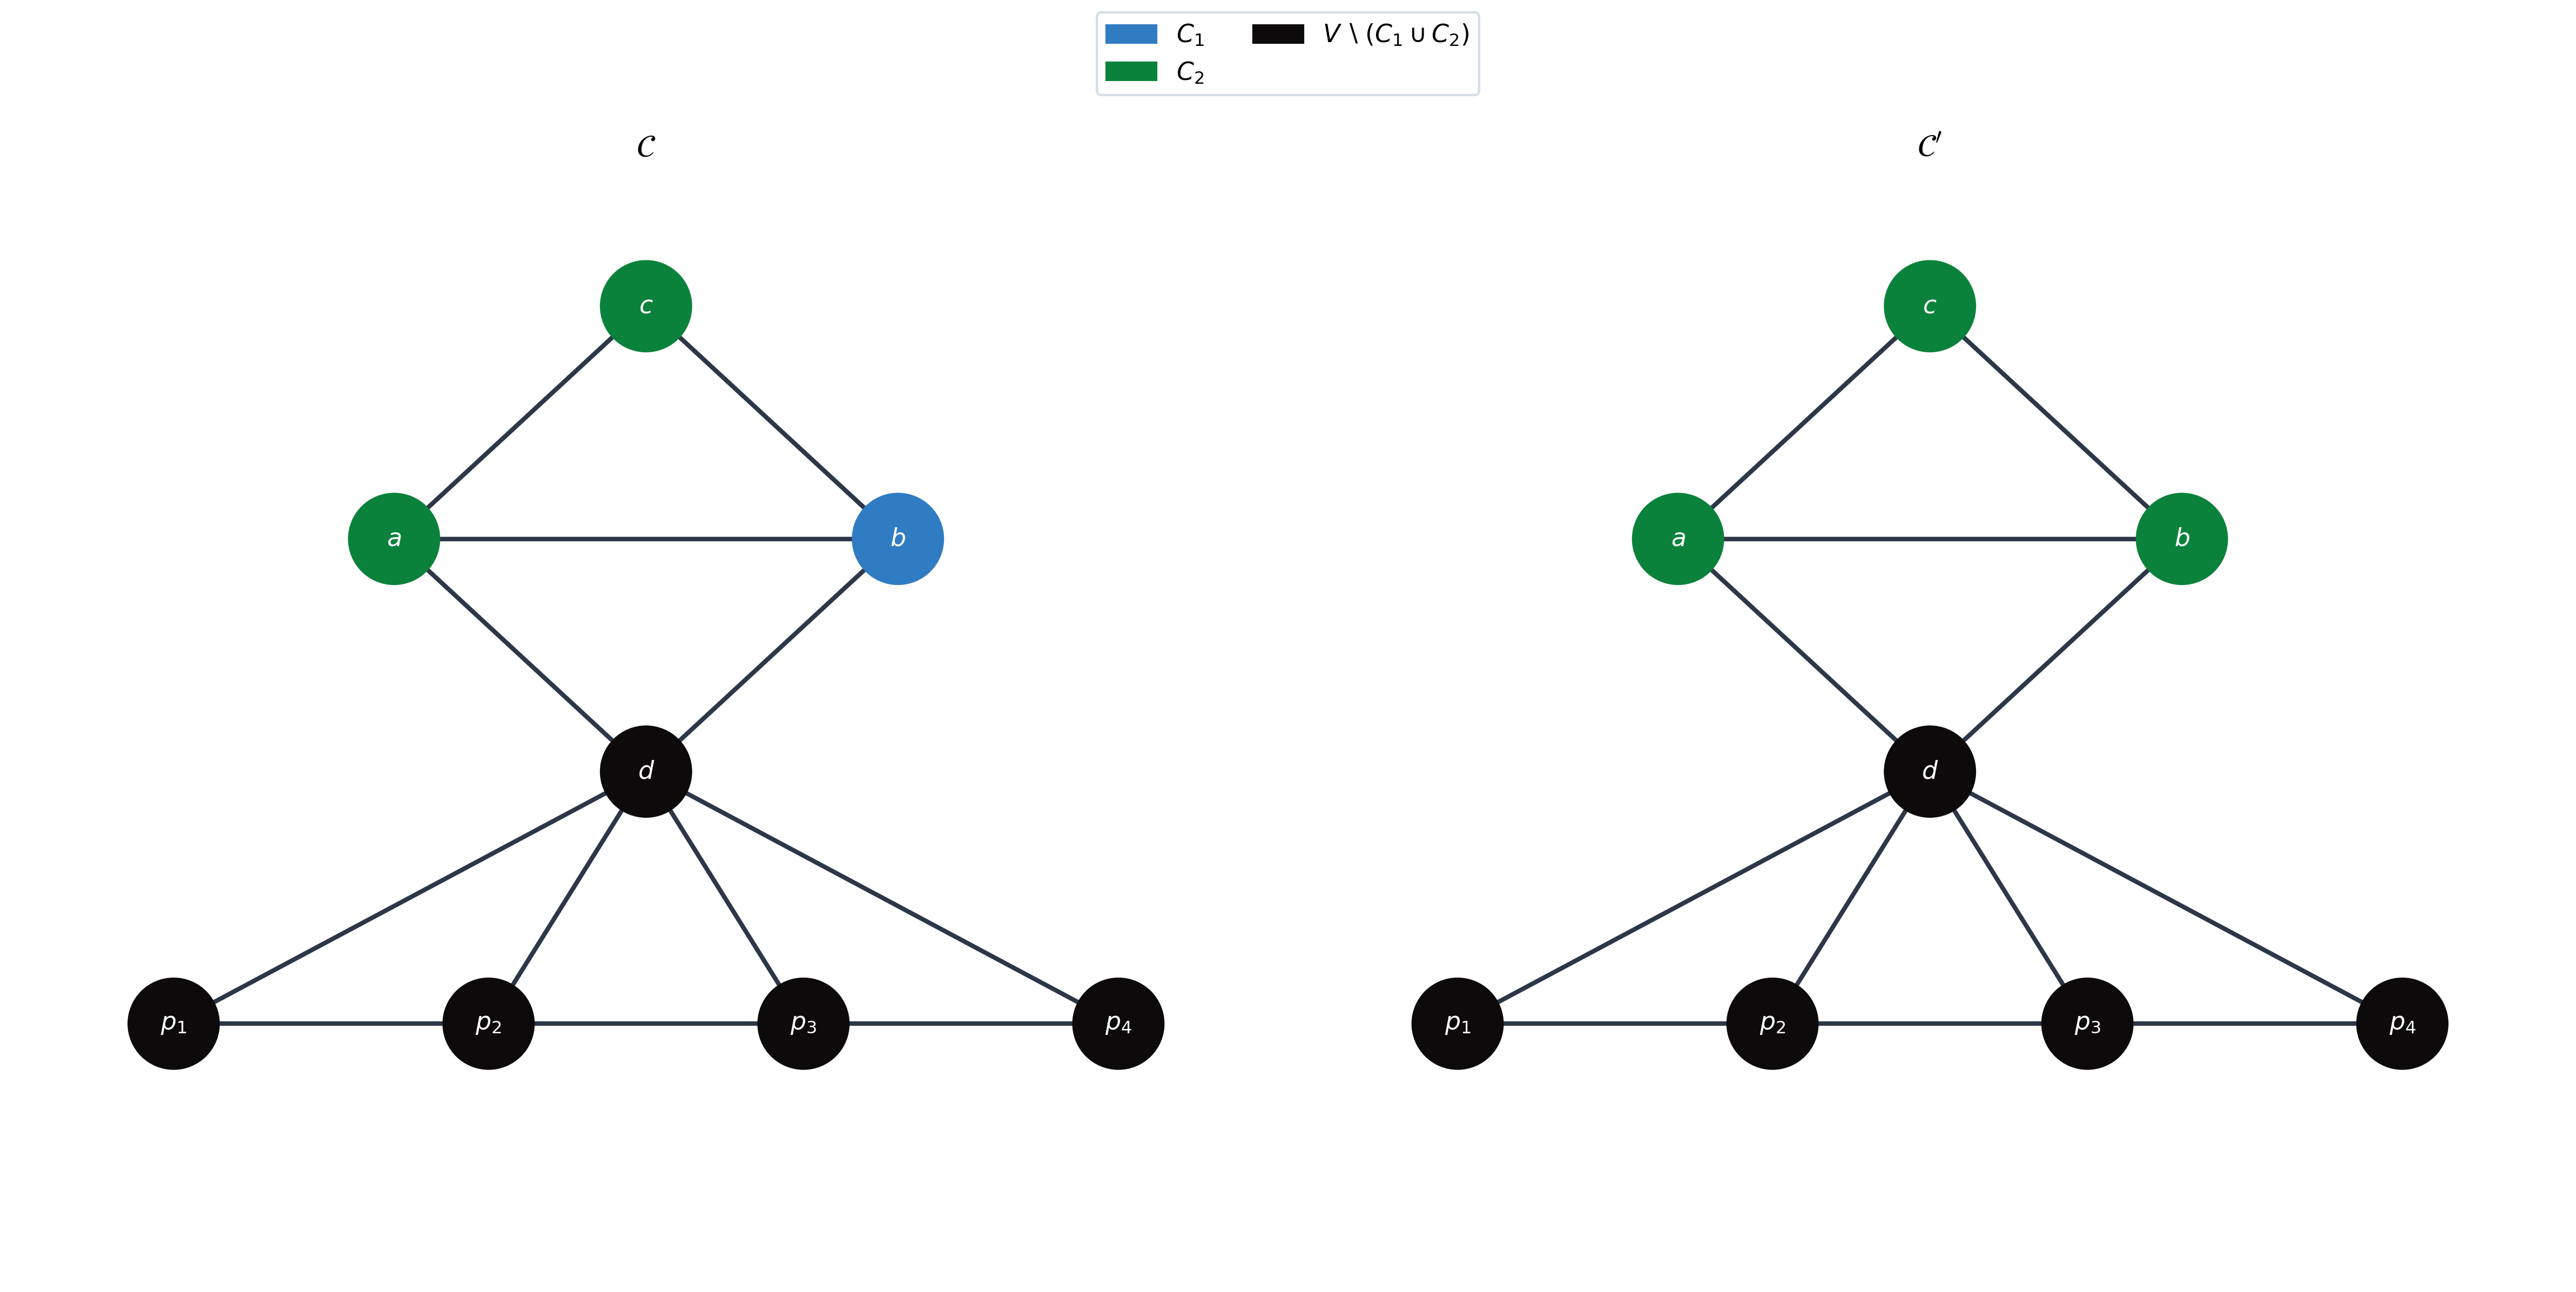
\includegraphics[width=0.7\textwidth]{../../graphs/t2c.png}
                              \caption{Moving b from its own cluster to the rest of the triangle.}
                              \label{fig:t2c}
                        \end{figure}
            \end{enumerate}
            Therefore, we can see that neither $a$ nor $b$ can be separated from the rest of its triangle. The last thing we need to show is that $c$ also cannot be separated.
      \item $a,b$ together, $c$ in its own one-vertex cluster.\\
            Let $C_1 = \{c\}, a,b \in C_2, C_1' = \emptyset$ and $C_2' = C_2 \cup \{c\}$. The difference is
            \begin{align*}
                   & \text{mod}_{\mathcal{C'}}(G) - \text{mod}_{\mathcal{C}} (G) \\
                   & = \frac{2}{m} - \frac{4vol(C_2)+4}{4m^2} + \frac{4}{4m^2}   \\
                   & = \frac{2m-vol(C_2)}{4m^2} > 0.                             \\
            \end{align*}
            \begin{figure}[H]
                  \centering
                  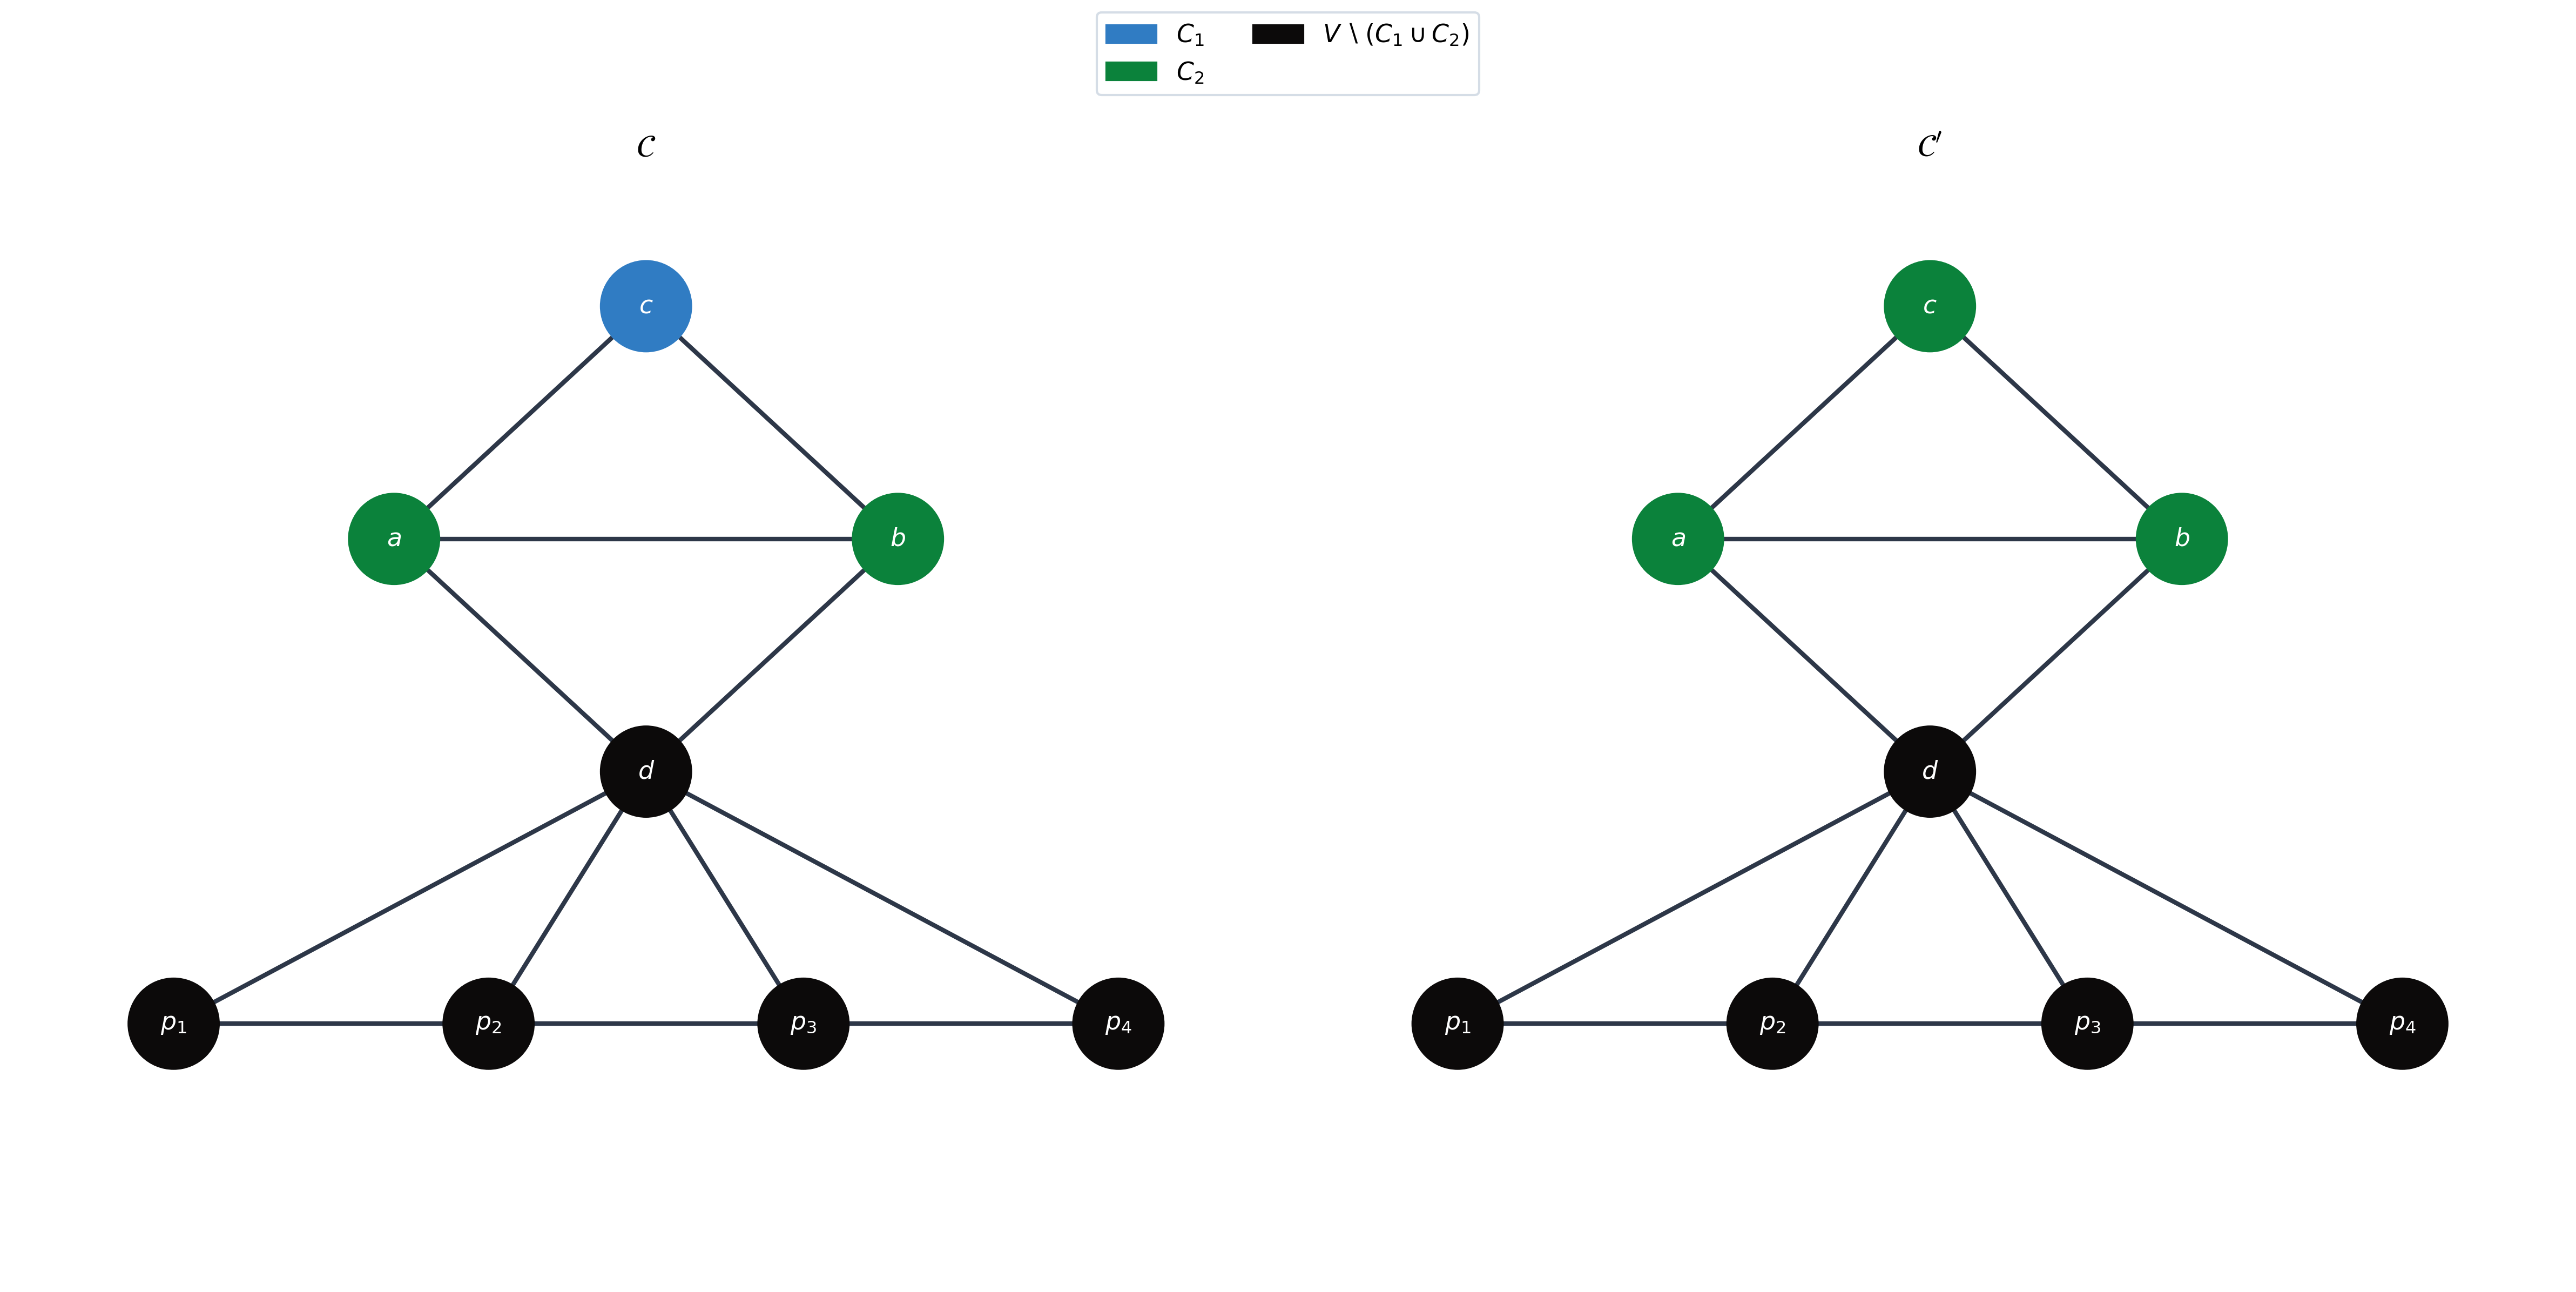
\includegraphics[width=0.7\textwidth]{../../graphs/t3.png}
                  \caption{Moving c to the rest of the triangle.}
                  \label{fig:t3}
            \end{figure}
            So, in optimal partitioning no triangle is split.
\end{enumerate}

The second question is: should we join the triangles with other vertices (excluding the connector)?

Let $\mathcal{C}$ and $\mathcal{C'}$ be clusterings such that $C_1, C_2 \in \mathcal{C}$ and $C'_1, C'_2 \in \mathcal{C'}$, where $C_1 = \{t_1\}$, $c_1 \notin C_2$, $C'_1 = \emptyset$, and $C'_2 = C_2 \cup \{t_{1}\}$.

Consider the difference
\begin{align*}
       & \text{mod}_{\mathcal{C'}}(G) - \text{mod}_{\mathcal{C}} (G)                                                \\
       & = -\frac{(\text{vol}(C_1) + \text{vol}(C_2))^2}{4m^2} + \frac{\text{vol}(C_1)^2 + \text{vol}(C_2)^2}{4m^2} \\
       & = - \frac{2\text{vol}(C_1)\text{vol}(C_2)}{4m^2} \leq 0.
\end{align*}

If the connector is taken away from the triangle (the diamond is split), then the triangle must be in its own community with no other vertices, so the answer is no.

Therefore, we need to consider only clusterings where the diamonds are not split, or where some connectors are grouped with path vertices and the remaining diamonds (whole or partial) remain in their own communities.

\subsection{Merging Intact Diamonds with Path Vertices}\label{merging_intact_diamonds_with_path_vertices}
Let $\mathcal{C}$ and $\mathcal{C'}$ be clusterings such that $C_1, C_2 \in \mathcal{C}$ and $C'_1, C'_2 \in \mathcal{C'}$, where $C_1 = \{d_{i1}, \ldots, d_{ij}\} \cup \{\text{$p$ vertices from the path}\}$, $C_2 = \{d_{k1}, \ldots, d_{kl}\}$, $C'_1 = C_1 \cup \{d_{k1}\}$, and $C'_2 = \{d_{k2}, \ldots, d_{kl}\}$.

We need to consider five different cases in terms of the presence of path vertices in the considered communities.

\begin{enumerate}
      \item $p = 0$\\
            First, we focus on the case where diamonds are in their own communities that do not contain path vertices.
            We have
            \begin{align*}
                   & \text{mod}_{\mathcal{C'}}(G) - \text{mod}_{\mathcal{C}} (G)                                                                                       \\
                   & = \frac{5}{m} - \frac{(\text{vol}(C_1)+14)^2 - \text{vol}(C_1)^2}{4m^2} - \frac{5}{m} - \frac{(\text{vol}(C_2) - 14)^2 - \text{vol}(C_2)^2}{4m^2} \\
                   & = \frac{28\text{vol}(C_2) - 28\text{vol}(C_1) - 392}{4m^2}                                                                                        \\
                   & = \frac{7\text{vol}(C_2) - 7\text{vol}(C_1) - 98}{m^2}                                                                                            \\
                   & = \frac{7\cdot 14 \cdot l - 7 \cdot 14 \cdot j - 98}{m^2}.
            \end{align*}

            Therefore, moving a diamond from a community with $l$ diamonds into one with $j$ diamonds (when neither contains a path vertex) is beneficial only if
            \[
                  7\cdot 14 \cdot l - 7 \cdot 14 \cdot j - 98 = l - j - 1 > 0.
            \]
            \textbf{Thus, we want to keep such communities as small as possible.} If we decide to create $9000$ diamond-communities, we can distinguish $3$ cases in terms of paths' communities. In the first case the whole path is in one community, such a clustering scores $0.50610928613506955820$. The second case is when there are two communities with two path vertices and it scores $0.53079470057896716018$. And the third case is when we have one community with one vertex and one community with $3$ vertices -- $0.52461957470893949562$.

      \item $p = 1$\\
            The difference in modularity scores is
            \begin{align*}
                   & \text{mod}_{\mathcal{C'}}(G) - \text{mod}_{\mathcal{C}} (G)                                                                                       \\
                   & = \frac{6}{m} - \frac{(\text{vol}(C_1)+14)^2 - \text{vol}(C_1)^2}{4m^2} - \frac{5}{m} - \frac{(\text{vol}(C_2) - 14)^2 - \text{vol}(C_2)^2}{4m^2} \\
                   & = \frac{1}{m} - \frac{28\text{vol}(C_1) - 28\text{vol}(C_2) + 392}{4m^2}                                                                          \\
                   & = \frac{7\text{vol}(C_2) - 7\text{vol}(C_1) - 98 + m}{m^2}.
            \end{align*}
            The inequality holds when
            \begin{align*}
                   & 7\text{vol}(C_2) - 7\text{vol}(C_1) - 98 + m > 0        \\
                   & \text{vol}(C_1) < \frac{m}{7} - 14 + \text{vol}(C_2)    \\
                   & 14 \cdot j + 9002(9001) < \frac{m}{7} - 14 + 14 \cdot l \\
                   & j < 182.56 + l.
            \end{align*}
            When a community contains one path vertex, in the best case it contains $184$ diamonds ($l = 1$, $j < 182.56 + 1 = 183.56$, moving one more gives $184$). In this case, the modularity score is $0.54413127767139846114$, which is the best score found.

      \item $p = 2$\\
            Moving a diamond to a community with two path vertices results in
            \begin{align*}
                   & \text{mod}_{\mathcal{C'}}(G) - \text{mod}_{\mathcal{C}} (G)                                                                                       \\
                   & = \frac{7}{m} - \frac{(\text{vol}(C_1)+14)^2 - \text{vol}(C_1)^2}{4m^2} - \frac{5}{m} - \frac{(\text{vol}(C_2) - 14)^2 - \text{vol}(C_2)^2}{4m^2} \\
                   & = \frac{2}{m} - \frac{28\text{vol}(C_1) - 28\text{vol}(C_2) + 392}{4m^2}                                                                          \\
                   & = \frac{7\text{vol}(C_2) - 7\text{vol}(C_1) - 98 + 2m}{m^2}.
            \end{align*}
            This is beneficial when
            \begin{align*}
                   & 7\text{vol}(C_2) - 7\text{vol}(C_1) - 98 + 2m > 0         \\
                   & \text{vol}(C_1) < \frac{2m}{7} - 14 + \text{vol}(C_2)     \\
                   & 14 \cdot j + 9002 + 9001 < \frac{2m}{7} - 14 + 14 \cdot l \\
                   & j < 366.12 + l.
            \end{align*}
            Therefore, the optimal community size here is $2$ path vertices plus $368$ ($=184 \cdot 2$) diamonds. The modularity score for this clustering is $0.53281397974556099495$.

      \item $p = 3$\\
            When one community contains $3$ path vertices, a second community must contain the remaining $1$. To find the optimal size of the receiving community, we apply the inequality from previous cases
            \begin{align*}
                   & 7\text{vol}(C_2) - 7\text{vol}(C_1) - 98 + 3m > 0     \\
                   & \text{vol}(C_1) < \frac{3m}{7} - 14 + \text{vol}(C_2) \\
                   & 14 \cdot j + 27005 < \frac{3m}{7} - 14 + 14 \cdot l   \\
                   & j < 549.76 + l.
            \end{align*}
            The modularity score for a partition with one community containing $3$ path vertices and $551$ diamonds, and another with $1$ path vertex and $184$ diamonds, is $0.52714210694891305842$.

      \item $p = 4$\\
            When the entire path is in one community, we can move diamonds to it as long as
            \begin{align*}
                   & 7\text{vol}(C_2) - 7\text{vol}(C_1) - 98 + 4m > 0     \\
                   & \text{vol}(C_1) < \frac{4m}{7} - 14 + \text{vol}(C_2) \\
                   & 14 \cdot j + 36006 < \frac{4m}{7} - 14 + 14 \cdot l   \\
                   & j < 733.39 + l.
            \end{align*}
            When the entire path community holds $735$ diamonds, the modularity score is $0.51014235729660872831$.
\end{enumerate}

Therefore, $p = 1$ is the optimal case. Joining two communities containing path fractions is not beneficial because $735 = 184\cdot 4 - 1$, $551 = 184 \cdot 3 - 1$, and $368 = 184 \cdot 2$.


\subsection{Possible Partitions}
Let us consider all possible partitions under an assumption that diamonds cannot be split. We can distinguish $5$ main cases in terms of the number of communities containing both path and diamond vertices, let $s$ be that number.

\begin{enumerate}
      \item $s=0$\\
            From Lemma \ref{connected_clusters} we know that clusters must induce connected subgraphs, therefore, there are $3$ options for clustering path vertices. The whole path is in one community or the path is split into two halves and there are two communities with two path vertices or there is one community with $3$ path vertices and one with $1$ vertex. However, all of these communities contributes negatively to mod score and from Lemma \ref{positive_score} we know that this cannot happen in optimal partitioning. So this case is not valid.\\
      \item $s=1$\\
            In this case, there is only one valid option -- the whole path must be in one community with some diamonds. Otherwise, there would be a community with a negative contribution (the previous case). We have already considered such clustering in Section \ref{merging_intact_diamonds_with_path_vertices} (case $5$).\\
      \item $s=2$\\
            There are $2$ options for path split to consider. The first is when both mixed communites contain $2$ path vertices, which is exactly case $3$ from Section \ref{merging_intact_diamonds_with_path_vertices}, and the second is when there is one cluster with $3$ and one with $1$ path vertex, which is exactly case $4$ from Section \ref{merging_intact_diamonds_with_path_vertices}. We do not need to consider selecting different vertices for specific communities because it will not improve the mod score. Path's vertices in one community must be connected to each other.\\
      \item $s=3$\\
            In this case, we should consider only the situation when there are two communities with $1$ path vertex and one with $2$ path vertices. Such clustering scores $0.53847262870847978355$ or $0.53847174643882433909$ depending on choosing the $2$ vertices to one community. That doesn't beat our best score.\\
      \item $s=4$\\
            The last case with the path being split into four communities is so far the best found one, considered in Case $2$ in Section \ref{merging_intact_diamonds_with_path_vertices}.
\end{enumerate}
Worth noting may be the fact that we don't need to consider moving diamonds between the communities containing path vertices. This is because we know the best sizes for such communities (from the calculations in the previous section) and in all cases we have some free diamonds left and we can use them to adjust each path cluster's size.

\subsection{Attachment of Isolated Connectors}
Let us analyze cases where connectors are placed in the path clusters to determine how many connectors should be added.

Let $\mathcal{C}$ and $\mathcal{C'}$ be clusterings with $C_1, C_2 \in \mathcal{C}$ and $C'_1, C'_2 \in \mathcal{C'}$.

\begin{enumerate}
      \item The entire path is in one community.\\
            Let $C_1 = \{d_1\}$, $\{p_1, p_2, p_3, p_4\} \in C_2$, $C'_1 = \{t_1\}$, $C'_2 = C_2 \cup \{c_1\}$, and let $c$ be the number of connectors in $C_2$.

            Calculating the modularity score difference
            \begin{align*}
                   & \text{mod}_{\mathcal{C'}}(G) - \text{mod}_{\mathcal{C}} (G)                                             \\
                   & = \frac{-2}{m} - \frac{-12\text{vol}(C_1) + 36}{4m^2} + \frac{4}{m} - \frac{12\text{vol}(C_2)+36}{4m^2} \\
                   & = \frac{2m + 3\text{vol}(C_1) - 3\text{vol}(C_2) - 18}{m^2}.
            \end{align*}
            Solving for $2m + 3\text{vol}(C_1) - 3\text{vol}(C_2) - 18 > 0$, we get
            \begin{align*}
                  \frac{2m}{3} + \text{vol}(C_1) - \text{vol}(C_2) - 6 & > 0                                  \\
                  \text{vol}(C_2)                                      & < \frac{2m}{3} - 6 + \text{vol}(C_1) \\
                  \text{vol}(C_2)                                      & < \frac{2\cdot 81003}{3} - 6 + 14    \\
                  36006 + 6c                                           & < 54010                              \\
                  c                                                    & < 3000.67.
            \end{align*}
            The optimal number of connectors in the community with the full path is $3001$. This clustering (with remaining diamonds in their own clusters) scores $0.51846365401584382226$.

      \item A community contains $2$ adjacent path vertices.\\
            Let $\{d_1\} \in C_1$, $\{p_1, p_2\} \in C_2$, $C'_1 = C_1 \setminus \{c_1\}$, $C'_2 = C_2 \cup \{c_1\}$, and $c$ be the number of connectors in $C_2$.

            The modularity change is
            \begin{align*}
                   & \text{mod}_{\mathcal{C'}}(G) - \text{mod}_{\mathcal{C}} (G)                                             \\
                   & = \frac{-2}{m} - \frac{-12\text{vol}(C_1) + 36}{4m^2} + \frac{2}{m} - \frac{12\text{vol}(C_2)+36}{4m^2} \\
                   & = \frac{3\text{vol}(C_1) - 3\text{vol}(C_2) - 18}{m^2}.
            \end{align*}
            Since $\text{vol}(C_2) \geq 18003$, the difference is positive only if $\text{vol}(C_1) > 18009$, requiring at least $1287$ diamonds. A clustering with $2$ communities of $1286$ diamonds and $1$ triangle, plus $2$ communities with path halves and $1$ connector, scores only $0.50607499809424871806$.

      \item A community contains one path vertex.\\
            Let $\{d_1\} \in C_1$, $\{p_1\} \in C_2$, $C'_1 = C_1 \setminus \{c_1\}$, $C'_2 = C_2 \cup \{c_1\}$, and $c$ be the number of connectors in $C_2$.

            The difference is
            \begin{align*}
                   & \text{mod}_{\mathcal{C'}}(G) - \text{mod}_{\mathcal{C}} (G) \\
                   & = \frac{3\text{vol}(C_1) - 3\text{vol}(C_2) - 18 - m}{m^2}.
            \end{align*}
            This case yields a lower score than Case 2 and cannot form the optimal clustering. Similarly, placing $3$ path vertices together and $1$ separately is inferior to Case 1.
\end{enumerate}

\subsection{Reassigning Connectors to Path Clusters}
Consider clustering $\mathcal{A}$. Moving connectors from $A_5, \ldots, A_{8268}$ to $A_1, \ldots, A_4$ yields the following result.

Let $C_1 = \{d_{i1}, \ldots, d_{ij}\} \cup \{\text{$p$ path vertices}\}$, $C_2 = \{d_{k1}, \ldots, d_{kl}\}$, $C'_1 = C_1 \cup \{c_{k1}\}$, and $C'_2 = C_2 \setminus \{c_{k1}\}$.

The difference in modularity score is
\begin{align*}
       & \text{mod}_{\mathcal{C'}}(G) - \text{mod}_{\mathcal{C}} (G)                                                                                     \\
       & = \frac{1}{m} - \frac{(\text{vol}(C_1)+6)^2 - \text{vol}(C_1)^2}{4m^2} - \frac{2}{m} - \frac{(\text{vol}(C_2) - 6)^2 - \text{vol}(C_2)^2}{4m^2} \\
       & = \frac{-1}{m} - \frac{12\text{vol}(C_1) - 12\text{vol}(C_2) + 72}{4m^2}                                                                        \\
       & = \frac{3\text{vol}(C_2) - 3\text{vol}(C_1) - 18 - m}{m^2}.
\end{align*}
Moving a connector from a free diamond is profitable only if $C_2$ is sufficiently large
\begin{align*}
       & 3\text{vol}(C_2) - 3\text{vol}(C_1) - 18 - m > 0    \\
       & \text{vol}(C_2) > \text{vol}(C_1) + 6 + \frac{m}{3} \\
       & \text{vol}(C_2) > 184 \cdot 14 + 9001 + 6 + 27001   \\
       & \text{vol}(C_2) > 38584 = 14 \cdot 2756.
\end{align*}
For this to hold, $C_2$ would need at least $2756$ free diamonds. However, that would contradict Lemma \ref{connected_clusters}, so cannot be optimal. A clustering with $2756$ diamonds missing one connector scores only $0.48742975922116960064$.

\section{Conclusions}
We have established the following.
\begin{enumerate}
      \item Triangles must always remain together in the same cluster.
      \item Any community containing a whole diamond without path vertices must contain only that single diamond.
      \item The optimal cluster sizes for path fractions and diamonds are identified ($p=1$ with $184$ diamonds).
      \item Splitting diamonds and placing isolated connectors into path communities yields suboptimal modularity scores.
      \item Moving connectors from unattached diamonds into path-fraction communities makes no sense.
\end{enumerate}

Since splitting diamonds optimally performs worse than $\mathcal{A}$, diamonds should remain intact and not merged without path vertices. Thus, $\mathcal{A}$ is the optimal partitioning, giving $\text{mod}(G) = 0.54413127767139846114$. This is strictly less than $0.55116544464653760560$ (the best found $\text{mod}^*$ score shown in Figure~\ref{mod_star}), proving that $\text{mod}(G) < \text{mod}^*(G)$ for graph $G$.

\begin{figure}[H]
      \centering
      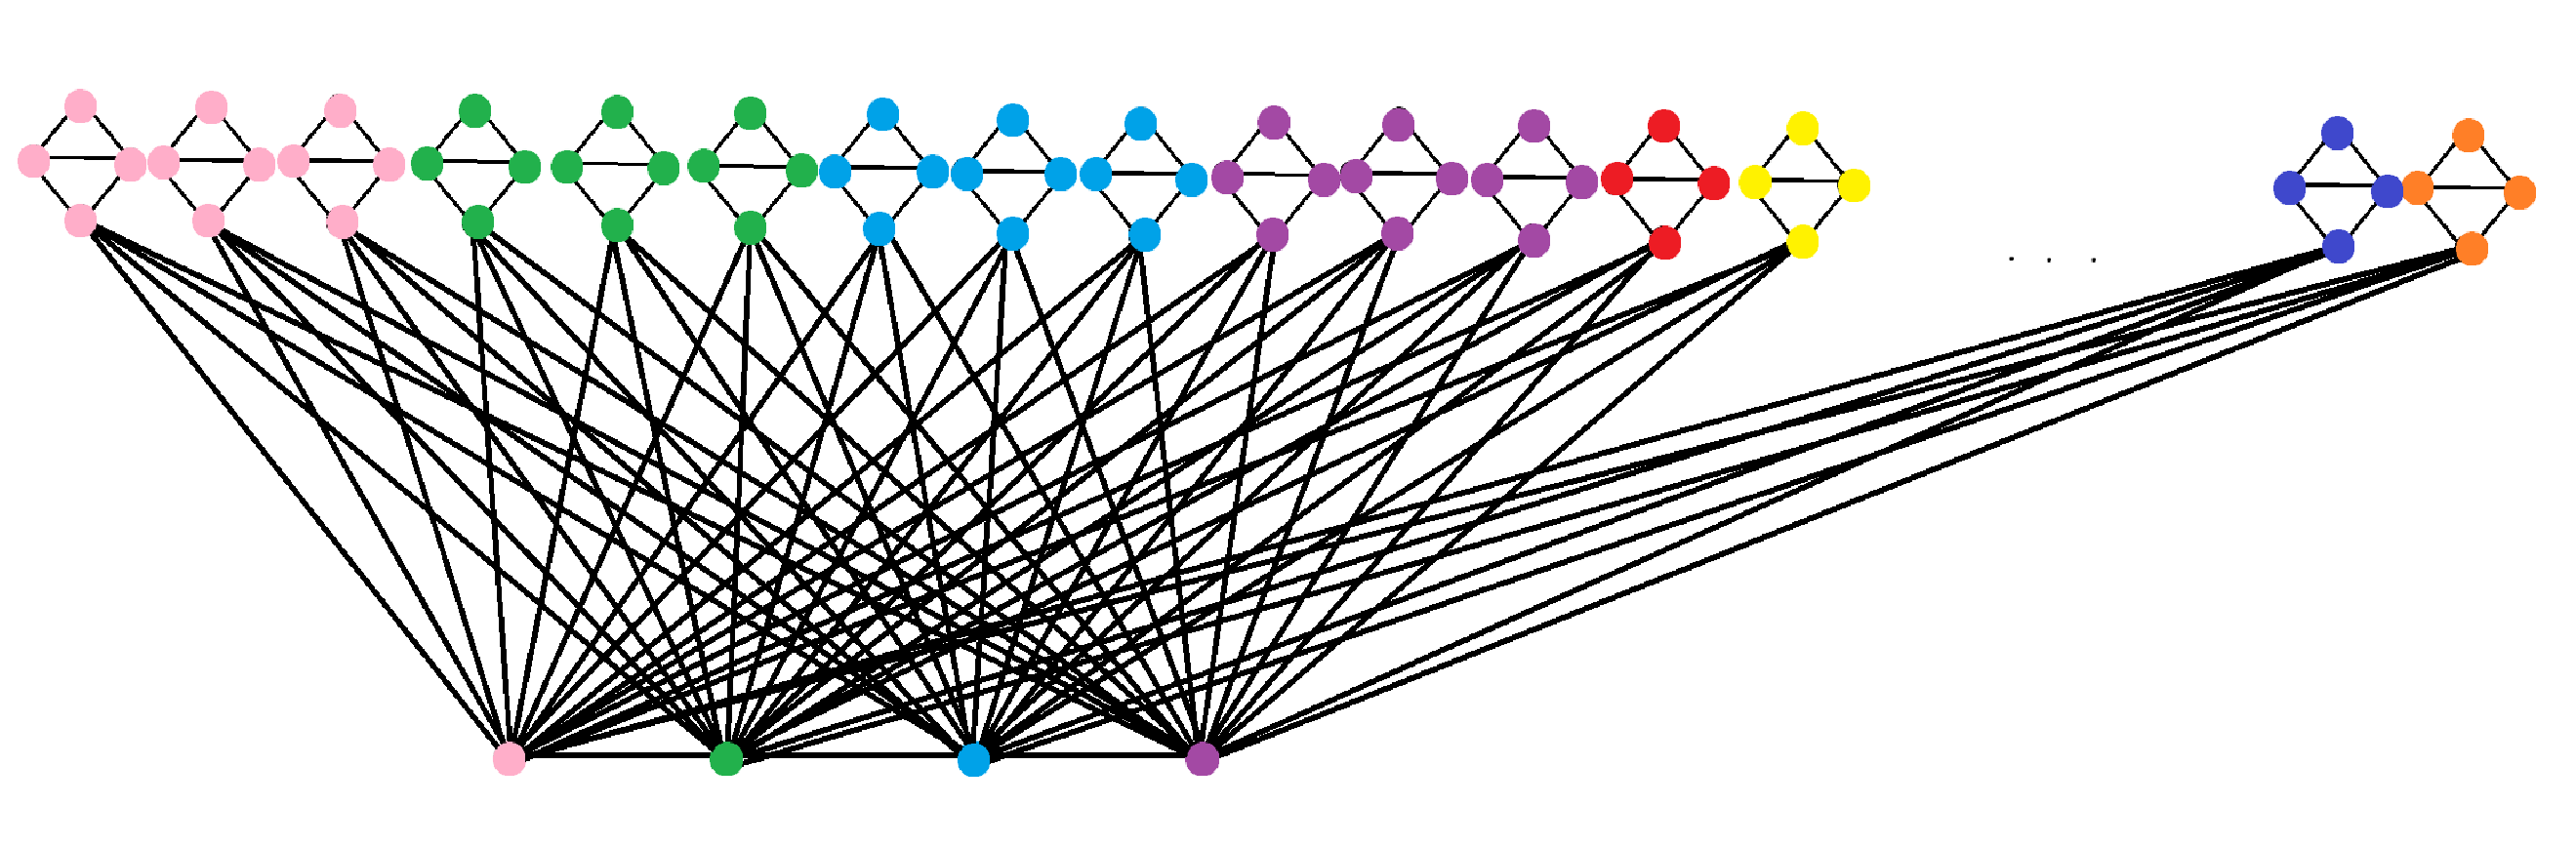
\includegraphics[width=0.9\textwidth]{../../graphs/mod_star.png}
      \caption{Diamond graph $G$, such that $\text{mod}^*(G) > \text{mod}(G)$.}
      \label{mod_star}
\end{figure}

\end{document}